%!TEX root = ../thesis.tex
%*******************************************************************************
%*********************************** Fourth Chapter *****************************
%*******************************************************************************

\chapter{Event Reconstruction from Test Beam Data}
\graphicspath{{4_Methods/Figs/}}

This chapter describes the test beam setup for data collection in this project, and outlines the procedures for extracting key physical quantities from the raw data - event reconstruction. 

%********************************** %First Section  **************************************
\section{Test Beam Setup} 
\label{section4.1}
In general, the time resolution of a sensor is determined by the width of the time residual distribution, which equals the difference between the arrival time of a particle at the sensor, $t_{dut}$, and a reference arrival time, $t_{ref}$:
\begin{equation}
    \Delta t_{residual} = t_{ref} - t_{dut}
    \label{eq:timeresidual}
\end{equation}

A test beam provides high-energy particles capable of traversing multiple sensor layers, allowing spatial and timing information to be measured across the setup. This enables track reconstruction and time comparison, making it essential for time resolution analysis.

The test beam measurement was performed at the DESY II, Germany, in March 2024 by Tianqi Gao et al\cite{testbeam}. The setup consists of four sensor planes and one scintillator, as shown in Fig. \ref{img:Telescope}. An electron beam of energy 4 GeV was passed through the setup.

\begin{figure}[h!]
\centering
\begin{subfigure}{.6\textwidth}
  \centering
  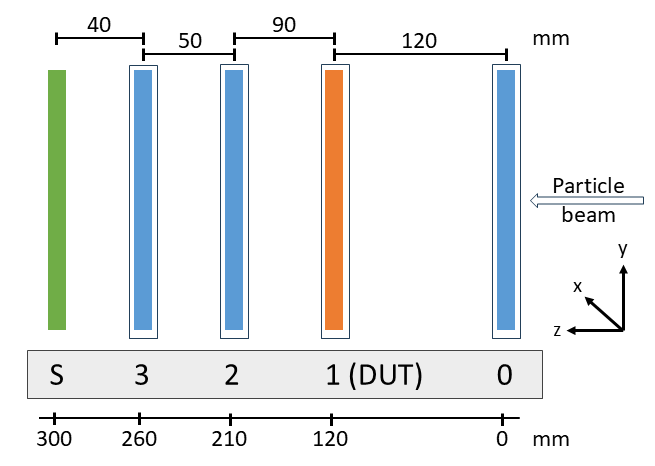
\includegraphics[width=1.0\linewidth]{Telescope}
  \caption{The telescope.}
  %\label{fig:sub1}
\end{subfigure}
\begin{subfigure}{.35\textwidth}
  \centering
  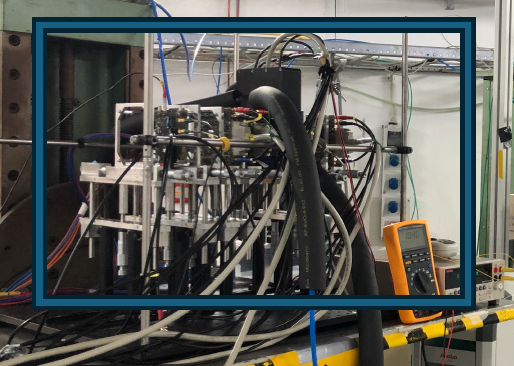
\includegraphics[width=1.0\linewidth]{Telescope_focus}
  \caption{A picture of the setup\cite{testbeam}.}
  %\label{fig:sub2}
\end{subfigure}
\caption{Schematic of the test beam setup. The orange layer represents the Device under Test (DUT), which is the TelePix2 sensor. Blue layers are the telescope layers, and the green layer is the scintillator. The rightmost (0th) layer serves as the reference layer.}
\label{img:Telescope}
\end{figure}

A MuPix11 telescope with MuDAQ readout was used. MuPix11 is a CMOS HV-MAPS that was designed for the Mu3e experiment, with a time resolution of 14.3 ns\cite{Mupix}, a spacial resolution of 23.1$\mu$m$\times$23.1$\mu$m and an active area of 256$\times$250 quadratic pixels of 80$\mu$m pitch\cite{Mupix2}. Similar to TelePix2, MuPix11 is capable of recording 2D spacial coordinates, ToA and ToT of the incoming signals. There are three MuPix11 planes in the telescope, where the first plane upstream serves as the reference plane. They provide reference spatial information for track reconstruction.

The Device under Test (DUT) - TelePix2 - was placed between the first and second MuPix11 plane. The scintillator was placed downstream and has a time resolution of approximately 1 ns. It provides ToA of the signal, because the time resolution of TelePix2 was expected to be better than that of the telescope.


%********************************** %Second Section  *************************************
\section{Event Reconstruction with Corryvreckan}
\label{section4.2}

A typical run in the experiment contains approximately $10^6$ hits on each of the five layers. To obtain a distribution of time residuals, it is essential to identify the path individual particles take through the setup. This is achieved through a process called event reconstruction, where coincidence events from different detector layers of the telescope are used to reconstruct the particle trajectory. It involves identifying spatially and temporally consistent hits across the layers, and grouping them into tracks. For test beams, the particles are usually highly relativistic, thus scattering is negligible and the tracks are taken to be straight lines. After a complete reconstruction, statistics can be gathered on the ToA difference between the DUT and the scintillator, by analysing a large number of individual particle tracks. 
%\footnote{There might be kinks at the detectors due to scattering processes. This can be taken into account by the General Broken Line (GBL) track model.}



%\begin{figure}[h!] 
%\centering    
%\includegraphics[width=0.6\linewidth]{Hitmap}
%\caption{A hit map of the reference plane of a typical run. The x,y axes represent the spatial coordinates, and the colour map represents the entries at each point. The entries are almost homogenous across the plane.}
%\label{img:Hitmap}
%\end{figure}



For the purpose of this project, the Corryvreckan framework\cite{Corry} was used for reconstruction. Corryvreckan is a 4D reconstruction and analysis software based on modern C++, initially developed by the CLICdp collaboration at CERN\cite{CLIC}. It is based on a modular design, where each step of the reconstruction process is performed separately by user-configurable modules. A flow chart of a typical Corryvreckan reconstruction chain is shown in Fig. \ref{img:CorryChain}. Each step will be briefly explained in the following. More detailed discussions on the architecture of the framework can be found in \cite{CorryIntro}\cite{CorryManual}\cite{CorryTutorial}.

%\begin{figure}[h!] 
%\centering    
%
\includegraphics[width=0.4\linewidth]{CorryLogo}
%\caption{The Corryvreckan framework\cite{Corry}.}
%\label{img:CorryLogo}
%\end{figure}

\begin{figure}[h!] 
\centering    
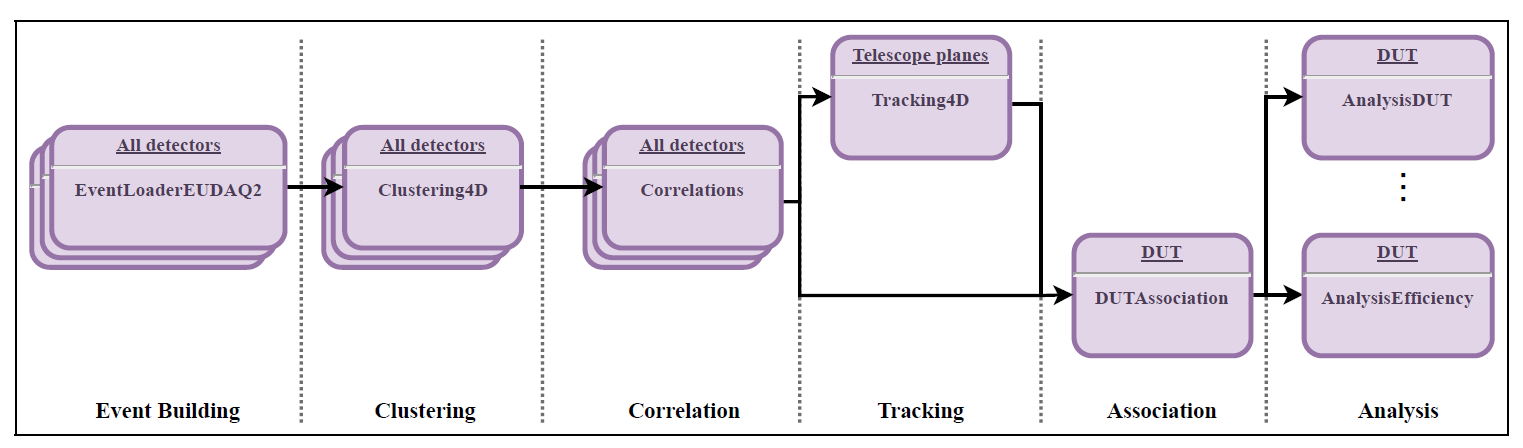
\includegraphics[width=1\linewidth]{CorryChain}
\caption{A typical Corryvreckan reconstruction process\cite{CorryIntro}. Each box represent a step in the reconstruction, which contains the corresponding Corryvreckan module. The underlined title refers to the sensor planes that the module applies to.}
\label{img:CorryChain}
\end{figure}

\subsection{Event Building}
The raw data files are coded in binary form. At the start of a reconstruction, decoding is needed for them to be processed by subsequent modules. This is performed by a group of modules called \texttt{EventLoader}. Here, for the MUDAQ readout, the corresponding \texttt{EventLoaderMupixTelescope} module was used.

 %Charge and hit-time calibrations are also applied at this stage, if needed. 

Next, the data is divided into time slices know as "events" to establish a unified time structure for all sensors. The event definition can vary depending on the purpose of the analysis\footnote{For a more detailed description of event definition based on individual detectors, see \cite{CorryIntro}.}. In this project, the \texttt{Metronome} module was used to define successive events of equal length 16$\mu$s, as illustrated in Fig. \ref{img:Metronome}. All subsequent modules obey this event definition, and provide only matching data\footnote{This is because the hit information are loaded onto the central clipboard storage on an event-basis, and the subsequent modules can only read information from the clipboard. In other words, the reconstruction steps are carried out within an event.}. 


\begin{figure}[h!] 
\centering    
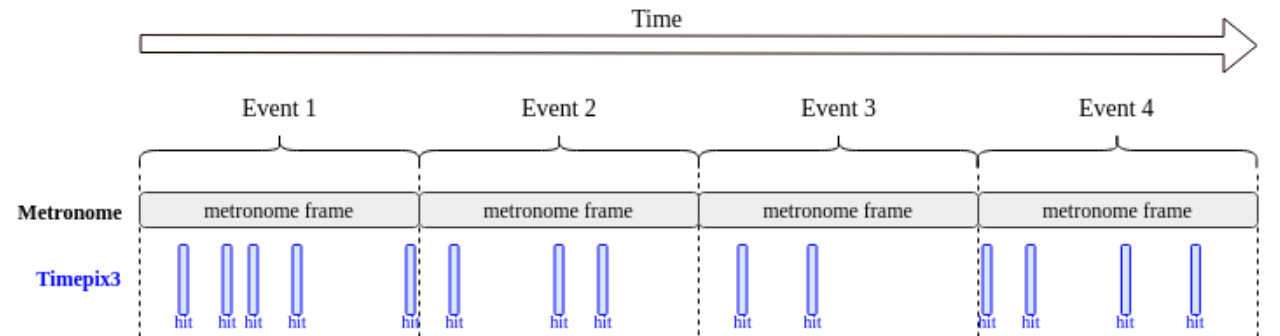
\includegraphics[width=1\linewidth]{Metronome}
\caption{The event building mechanism based on \texttt{Metronome}\cite{CorryTutorial}. It defines the events, and the subsequent \texttt{EventLoaderTimepix3} module loads all signals with suitable timestamp to the central clipboard storage.}
\label{img:Metronome}
\end{figure}

\subsection{Clustering}
A cluster is a collection of adjacent pixel hits that originate from a single traversing particle, due to charge sharing. Clustering is the process of identifying and grouping the hits into clusters. The \texttt{Clustering4D} module performs a nearest-neighbour search for all pixel hits on a sensor plane, and produces clusters accordingly. This is performed for all sensor planes. The cluster position is determined by taking the arithmetic mean of pixel hit positions within the cluster. The cluster timestamp is taken to be the timestamp of the highest-charge pixel. The charge of the cluster is the sum of pixel charges.



\subsection{Track fitting}
There are two steps in the track fitting process: the first is to find all possible track candidates using one of the \texttt{Tracking} modules; The second is to perform fitting with the track object, where bad fits are discarded and the result is reported back to the module.

The \texttt{Tracking4D} module was chosen for the process. For every signal detected on the first (upstream) sensor plane and each signal on the last plane, a straight line is connected between them - which is a primary track candidate. It is then possible to determine where and when the track candidate intercepts with the remaining planes. 

Next, the module searches for clusters on these remaining telescope planes that are within a configurable spatial and time window\footnote{The time window should be dependent of the distances between layers. However, the Time of Flight is usually in the order of $10^9$s and negligible comparing to time cut.}. In this analysis, the windows were set to be 500$\mu$m$\times$500$\mu$m and 200 ns for good statistics. Only when matching clusters are found on all telescope planes, a track can be assigned to these signals. %If multiple clusters satisfy the condition, the one closest (spacially) to the intersection point is chosen. Notice that if one cluster is associated to more than one tracks, then only the track with lowest $\chi$ value will be kept.

Finally, the remaining tracks are added to the clipboard. Each track timestamp is calculated by the average timestamp from all clusters in the track. %The track time relative to the start of the event and the residuals in positions are calculated.

\begin{figure}[h!] 
\centering    
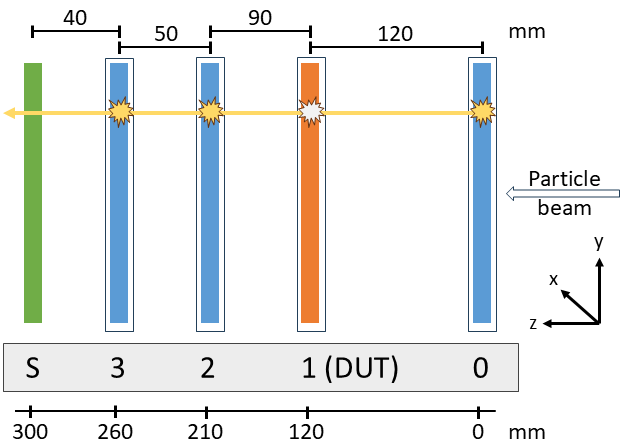
\includegraphics[width=0.6\linewidth]{Tracking}
\caption{Schematic of fitting of a straight track. The track is marked as an yellow arrow. The yellow clusters are those responsible for fitting the track. The white cluster is the DUT cluster that is associated to this track. }
\label{img:Tracking}
\end{figure}


\subsection{Association of DUT Clusters with Tracks}
After track constructions, the \texttt{DUTAssociation} module searches for clusters on the DUT around the intersection point of each track. Analogous to \texttt{Tracking4D}, clusters within the spatial and temporal cut, which was chosen to be 500$\mu$m$\times$500$\mu$m and 500 ns respectively, will be associated to the track. 

%Due to the mismatch between telescope sensor size(256$\times$250 of 80$\mu$m$\times$80$\mu$m pixels) and DUT size(120$\times$400 of 165$\mu$m$\times$25$\mu$m pixels), only about half of the tracks pass through the active area of the DUT. 
The efficiency of the DUT can be calculated from these tracks:

\begin{equation}
    \text{Efficiency} = \frac{\# \text{tracks with associated clusters on DUT}}{\# \text{total tracks through DUT}}.
    \label{eq:Efficiency}
\end{equation}


%%% If not moved, put the alignment section back here!!




\subsection{Analysis of the DUT}

Before the final analysis, corrections to the setup geometry are required, as it was measured manually at the test beam. A detailed description of the alignment procedure is provided in Appendix \ref{appendix:align}. Once the telescope and DUT have been successfully aligned, the reconstructed data can be considered reliable and used for subsequent analysis.

The \texttt{AnalysisEfficiency} and \texttt{AnalysisDUT} modules perform analysis and calculate key quantities about the performance of the DUT, such as efficiency and time resolution. Most Corryvreckan modules generate ROOT histograms\cite{ROOT}, from which analysis plots can be directly accessed.



%********************************** %Third Section  *************************************
\subsection{Correction for Time-walk Effect}
\label{section:timewalk}

In this project, correction for the time-walk effect is calculated by a stand-alone python file developed by Mary Richardson-Slipper et al\cite{MaryRepos}. For each Time-over-Threshold(ToT) value, a vertical slice is taken from the 2D histogram of time residual versus ToA. The width of the slice was set to be 20 ns, to balance fitting accuracy and statistics. %Narrower slices result in low statistics, leading to unstable fits. Conversely, wider slices provide sufficient statistics, but fail to capture the change in time residual, particularly at low ToT where the variation is rapidly changing.

Each slice is then projected on to the time residual (y) axis, giving a 1D histogram of time residual, as shown in Fig. \ref{img:CorrectionSlice}. A crystal ball function is fitted to the distribution, and the mean of the fit is taken as the correction value for that ToT. To validate the correction, the fitted values are compared against an empirical model for the time-walk effect\cite{Timewalk}:
\begin{equation}
\Delta t_{timewalk} = \frac{a}{(E+b)^d}+c
    \label{eq:Timewalk}
\end{equation}
where $E$ denotes the ToT, and $a,b,c,d$ are fit parameters. 

\begin{figure}[h!] 
\centering    
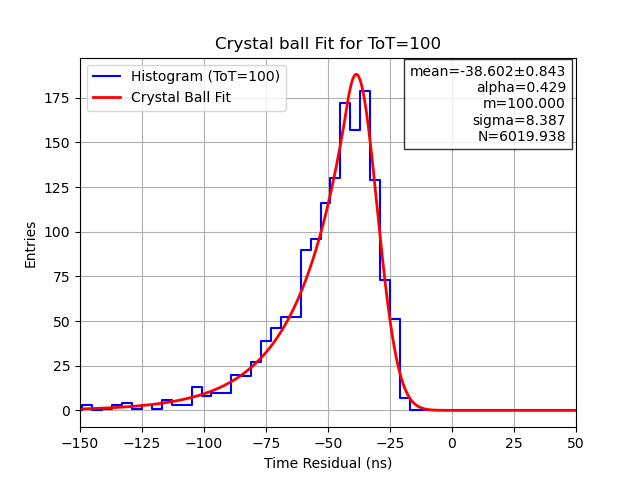
\includegraphics[width=.7\linewidth]{CorrectionSlice}
\caption{An example crystal ball fit, for a slice of width 20 ns at ToT=100 ns, from Fig. \ref{img:BeforeCorrection}. The correction for this ToT value is taken to be the fitted mean value, -38.602 ns.}
\label{img:CorrectionSlice}
\end{figure}


\begin{figure}[h!] 
\centering    
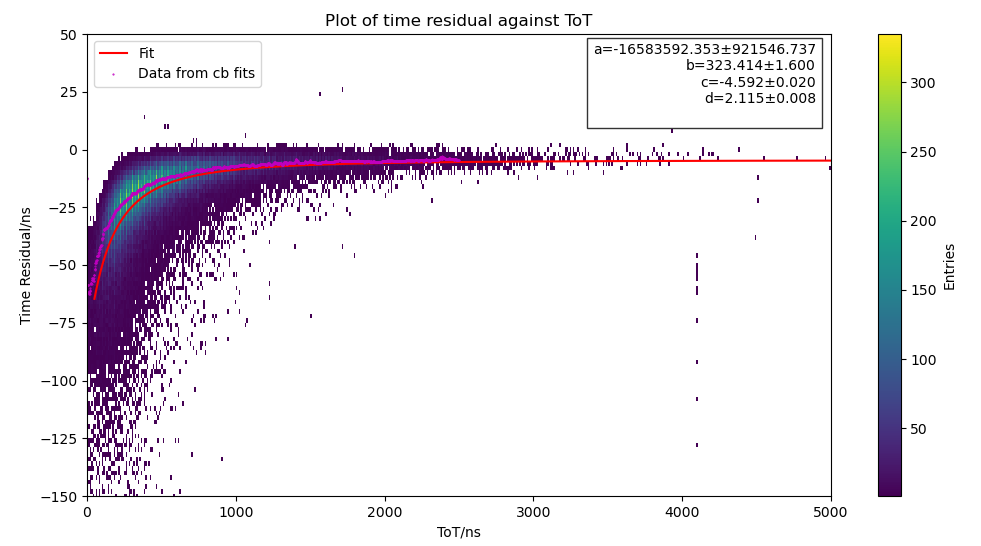
\includegraphics[width=1\linewidth]{BeforeCorrection}
\caption{An example plot of time residual versus Time-over-Threshold(ToT), where the colour map represent the entries at each point. The curvature at low ToT values illustrates the time-walk effect. Purple markers refers to the correction values calculated from crystal ball fits, while the red curve is a fit to Eq. \ref{eq:Timewalk}. Both methods yield a consistent trend with slight deviations at low ToT values. Note that the threshold in this run was 200 DAC, which is significantly higher than typical values used in data-taking - purely to emphasis the time-walk effect.}
\label{img:BeforeCorrection}
\end{figure}

It is worth noting that at high ToT values, the time residuals are not centred at zero. This offset arises from a constant time difference between the DUT and scintillator timestamps. The correction method described here have accounted for both this offset and the time-walk effect.

%The \texttt{AnalysisTimingATLASpix} module can also be used to compute time-walk correction, but it relies on Gaussian fit, which is found to be less accurate - particularly at low ToT values. The difference between the Gaussian mean and the Crystal Ball mean can reach up to 1ns. Therefore, in this project, \texttt{AnalysisTimingATLASpix} was used only to write the externally calculated correction values into Corryvreckan objects, such as pixels and clusters.
